%LTeX: language=it
\subsection{UC 1 - Inviare un'e-mail} \label{sec:UC1}
    \begin{figure}[h]
        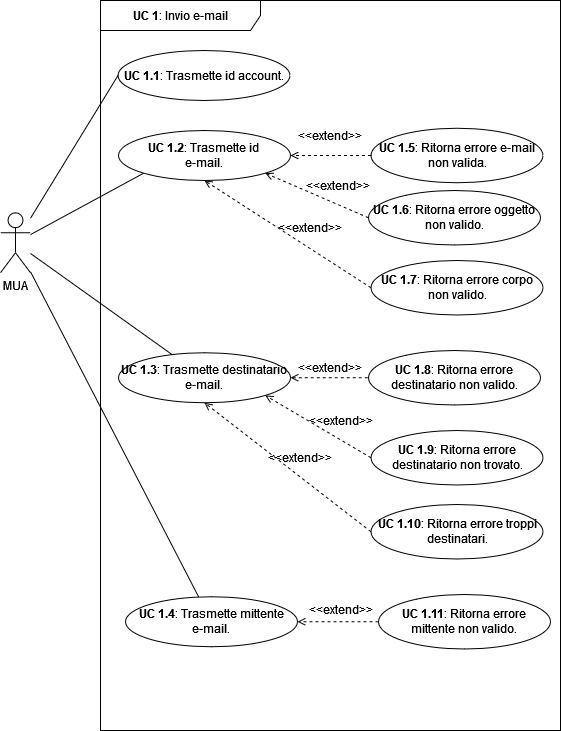
\includegraphics[width=0.85\textwidth]{sections/uc_imgs/UC01.png}
        \centering
        \caption{Diagramma UC 1.}
    \end{figure}
    \begin{itemize}
        \item \textbf{Attore principale}: MUA;
        \item \textbf{Descrizione}: il MUA deve poter inviare una e-mail al destinatario indicato;
        \item \textbf{Precondizioni}: l’account che il MUA gestisce è registrato nel sistema, e ha un connessione aperta con il sistema ed è autenticato;
        \item \textbf{Postcondizioni}: l'e-mail è stata consegnata con successo al destinatario, ed è stata salvata nel sistema;
        \item \textbf{Scenario principale}:
            \begin{enumerate}
                \item il MUA trasmette il destinatario dell'e-mail (\hyperref[sec:UC1.1]{UC 1.1});
                \item il MUA trasmette il mittente dell'e-mail (\hyperref[sec:UC1.2]{UC 1.2});
                \item il MUA trasmette l'oggetto dell'e-mail (\hyperref[sec:UC1.3]{UC 1.3});
                \item il MUA trasmette il corpo dell'e-mail (\hyperref[sec:UC1.4]{UC 1.4});
                \item il sistema elabora l'inoltro;
            \end{enumerate}
        \item \textbf{Inclusioni}: nessuna;
        \item \textbf{Generalizzazioni}: nessuna;
        \item \textbf{Estensioni}: 
            \begin{enumerate}[label=\alph*.]
                \item il sistema incontra un errore durante il tentativo d'invio dell'e-mail:
                \begin{enumerate}[label=\arabic*.]
                    \item invia l'e-mail con il codice d'errore al MUA (\hyperref[sec:UC2]{UC 2}).
                \end{enumerate}
            \end{enumerate}
    \end{itemize}

    \begin{figure}[h]
        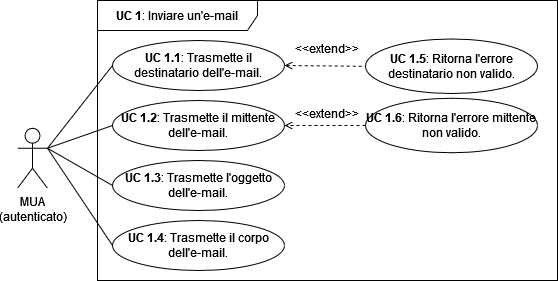
\includegraphics[width=0.75\textwidth]{sections/uc_imgs/UC01.X.png}
        \centering
        \caption{Diagramma sotto-casi UC 1.}
    \end{figure}

    \subsubsection{UC 1.1 - Trasmettere il destinatario dell'e-mail} \label{sec:UC1.1}
    \begin{itemize}
        \item \textbf{Attore}: MUA;
        \item \textbf{Descrizione}: il MUA invia al sistema il destinatario dell'e-mail;
        \item \textbf{Precondizioni}: il MUA sta usando la funzionalità d'invio di un'e-mail;
        \item \textbf{Postcondizioni}: il sistema conosce l'indirizzo di posta elettronica del destinatario dell'e-mail;
        \item \textbf{Scenario principale}:
            \begin{enumerate}
                \item il MUA trasmette il destinatario, deve soddisfare il seguente requisito:
                    \begin{itemize}
                        \item l'indirizzo e-mail deve essere sintatticamente valido;
                    \end{itemize}
            \end{enumerate}
        \item \textbf{Inclusioni}: nessuna;
        \item \textbf{Generalizzazioni}: nessuna;
        \item \textbf{Estensioni}:
            \begin{enumerate}[label=\alph*.]
                \item l'indirizzo e-mail non è sintatticamente valido:
                \begin{enumerate}[label=\arabic*.]
                    \item il sistema invia un messaggio di errore al MUA (\hyperref[sec:UC1.6]{UC 1.6}).
                \end{enumerate}
            \end{enumerate}
    \end{itemize}

    \subsubsection{UC 1.2 - Trasmettere il mittente dell'e-mail} \label{sec:UC1.2}
    \begin{itemize}
        \item \textbf{Attore}: MUA;
        \item \textbf{Descrizione}: il MUA invia al sistema il mittente dell'e-mail;
        \item \textbf{Precondizioni}: il MUA sta usando la funzionalità d'invio di un'e-mail;
        \item \textbf{Postcondizioni}: il sistema conosce l'indirizzo di posta elettronica del mittente dell'e-mail;
        \item \textbf{Scenario principale}:
            \begin{enumerate}
                \item il MUA trasmette il mittente, deve soddisfare il seguente requisito:
                    \begin{itemize}
                        \item l'indirizzo e-mail deve essere sintatticamente valido;
                    \end{itemize}
            \end{enumerate}
        \item \textbf{Inclusioni}: nessuna;
        \item \textbf{Generalizzazioni}: nessuna;
        \item \textbf{Estensioni}:
            \begin{enumerate}[label=\alph*.]
                \item l'indirizzo e-mail non è sintatticamente valido:
                \begin{enumerate}[label=\arabic*.]
                    \item il sistema invia un messaggio di errore al MUA (\hyperref[sec:UC1.7]{UC 1.7}).
                \end{enumerate}
            \end{enumerate}
    \end{itemize}

    \subsubsection{UC 1.3 - Trasmettere l'oggetto dell'e-mail} \label{sec:UC1.3}
    \begin{itemize}
        \item \textbf{Attore}: MUA;
        \item \textbf{Descrizione}: il MUA invia al sistema l'oggetto dell'e-mail;
        \item \textbf{Precondizioni}: il MUA sta usando la funzionalità d'invio di un'e-mail;
        \item \textbf{Postcondizioni}: il sistema conosce l'oggetto dell'e-mail;
        \item \textbf{Scenario principale}:
            \begin{enumerate}
                \item il MUA trasmette l'oggetto dell'e-mail;
            \end{enumerate}
        \item \textbf{Inclusioni}: nessuna;
        \item \textbf{Generalizzazioni}: nessuna;
        \item \textbf{Estensioni}: nessuna.
    \end{itemize}

    \subsubsection{UC 1.4 - Trasmettere il corpo dell'e-mail} \label{sec:UC1.4}
    \begin{itemize}
        \item \textbf{Attore}: MUA;
        \item \textbf{Descrizione}: il MUA invia al sistema il corpo dell'e-mail;
        \item \textbf{Precondizioni}: il MUA sta usando la funzionalità d'invio di un'e-mail;
        \item \textbf{Postcondizioni}: il sistema conosce il corpo dell'e-mail;
        \item \textbf{Scenario principale}:
            \begin{enumerate}
                \item il MUA trasmette il corpo dell'e-mail;
            \end{enumerate}
        \item \textbf{Inclusioni}: nessuna;
        \item \textbf{Generalizzazioni}: nessuna;
        \item \textbf{Estensioni}: nessuna.
    \end{itemize}

    % \subsubsection{UC 1.5 - Trasmettere gli allegati dell'e-mail} \label{sec:UC1.5}
    % \begin{itemize}
    %     \item \textbf{Attore}: MUA;
    %     \item \textbf{Descrizione}: il MUA invia al sistema il mittente dell'e-mail;
    %     \item \textbf{Precondizioni}: il MUA sta usando la funzionalità d'invio di un'e-mail;
    %     \item \textbf{Postcondizioni}: il sistema conosce l'indirizzo di posta elettronica del mittente dell'e-mail;
    %     \item \textbf{Scenario principale}:
    %         \begin{enumerate}
    %             \item il MUA trasmette gli allegati;
    %         \end{enumerate}
    %     \item \textbf{Inclusioni}: nessuna;
    %     \item \textbf{Generalizzazioni}: nessuna;
    %     \item \textbf{Estensioni}: 
    %         \begin{enumerate}[label=\alph*.]
    %             \item l'allegato supera la dimensione massima supporta dal sistema:
    %                 \begin{enumerate}[label=\arabic*.]
    %                     \item il sistema invia un messaggio di errore al MUA (\hyperref[sec:UC1.6]{UC 1.6}).
    %                 \end{enumerate}
    %         \end{enumerate}
    % \end{itemize}

    \subsubsection{UC 1.5 - Ritorna l'errore destinatario non valido} \label{sec:UC1.5}
    \begin{itemize}
        \item \textbf{Attore}: MUA;
        \item \textbf{Descrizione}: il MUA riceve l'errore che il destinatario non è valido;
        \item \textbf{Precondizioni}: il MUA ha inviato il destinatario;
        \item \textbf{Postcondizioni}: il MUA viene notificato che il destinatario non è valido;
        \item \textbf{Scenario principale}:
            \begin{enumerate}
                \item il sistema controlla la sintassi del destinatario e trova un errore;
                \item il sistema notifica il MUA che il destinatario non è valido;
            \end{enumerate}
        \item \textbf{Inclusioni}: nessuna;
        \item \textbf{Generalizzazioni}: nessuna;
        \item \textbf{Estensioni}: nessuna.
    \end{itemize}

    \subsubsection{UC 1.6 - Ritorna l'errore mittente non valido} \label{sec:UC1.6}
    \begin{itemize}
        \item \textbf{Attore}: MUA;
        \item \textbf{Descrizione}: il MUA riceve l'errore che il mittente non è valido;
        \item \textbf{Precondizioni}: il MUA ha inviato il mittente;
        \item \textbf{Postcondizioni}: il MUA viene notificato che il mittente non è valido;
        \item \textbf{Scenario principale}:
            \begin{enumerate}
                \item il sistema controlla la sintassi del mittente e trova un errore;
                \item il sistema notifica il MUA che il mittente non è valido;
            \end{enumerate}
        \item \textbf{Inclusioni}: nessuna;
        \item \textbf{Generalizzazioni}: nessuna;
        \item \textbf{Estensioni}: nessuna.
    \end{itemize}

    % \subsubsection{UC 1.8 - Ritorna l'errore massima dimensione allegati} \label{sec:UC1.8}
    % \begin{itemize}
    %     \item \textbf{Attore}: MUA;
    %     \item \textbf{Descrizione}: il MUA viene notificato che gli allegati dell'e-mail hanno superato la massima dimensione supportata;
    %     \item \textbf{Precondizioni}: il MUA sta usando di trasmissione degli allegati;
    %     \item \textbf{Postcondizioni}: il MUA è stato notificato del superamento della massima dimensione per gli allegati;
    %     \item \textbf{Scenario principale}:
    %         \begin{enumerate}
    %             \item il sistema controlla la dimensione degli allegati;
    %             \item il sistema nota che la dimensione è stata superata;
    %             \item il sistema notifica il MUA che la dimensione degli allegati supera la massima dimensione consentita per un e-mail;
    %         \end{enumerate}
    %     \item \textbf{Inclusioni}: nessuna;
    %     \item \textbf{Generalizzazioni}: nessuna;
    %     \item \textbf{Estensioni}: nessuna.
    % \end{itemize}